\documentclass[twocolumn,amsmath,amssymb,prl]{revtex4-1}
\usepackage{graphicx}% Include figure files
\usepackage{dcolumn}% Align table columns on decimal point
\usepackage{bm}% bold math
\usepackage{color}

%%%%%%%%%%%%%%%%%%%%%%%%%%%%%%%%%%%%%%%%%%%%%%%%%%%%%%%%%%%%
%% Definitions
\def\re{\text{Re}}
\def\im{\text{Im}}
\def\ket#1{\vert #1 \rangle}
\def\cU{{\cal{U}}}
\def\cD{{\cal{D}}}
\def\re{\text{Re}}
\def\im{\text{Im}}
\newcommand{\red}[1]{{\bf \color{red} #1}}
\newcommand{\blue}[1]{{\bf \color{blue} #1}}
\newcommand{\green}[1]{{\bf \color{green} #1}}
\newcommand{\rr}{\textbf{r}}
\newcommand{\xx}{\textbf{r}}
\newcommand{\refnote}{\red{[ref]}}

\newcommand\etadisp{\ensuremath{\eta_\textit{d}}}
\newcommand\epsilondisp{\ensuremath{\epsilon_\textit{d}}}
\newcommand\epsilonassoc{\ensuremath{\epsilon_\textit{a}}}
\newcommand\kappaassoc{\ensuremath{\kappa_\textit{a}}}
\newcommand\lambdadisp{\ensuremath{\lambda_\textit{d}}}
\newcommand\lscale{\ensuremath{s_d}}

% fixme is intended to prioritize stuff that needs fixing.
\newcommand{\fixme}[1]{\textcolor{red}{[\emph{#1}]}}

%%%%%%%%%%%%%%%%%%%%%%%%%%%%%%%%%%%%%%%%%%%%%%%%%%%%%%%%%%%%

\begin{document}
\title{A Classical Density-Functional Theory for Describing Water Interfaces}

\author{Eric J. Krebs}
\affiliation{Department of Physics, Oregon State University,
  Corvallis, OR 97331, USA}
\author{Jeff B. Schulte}
\affiliation{Department of Physics, Oregon State University,
  Corvallis, OR 97331, USA}
\author{David Roundy}
\affiliation{Department of Physics, Oregon State University,
  Corvallis, OR 97331, USA}

\begin{abstract}
We develop an improved version of our old functional.
\end{abstract}
\maketitle

\section{Introduction}

Water, the universal solvent, is of critical practical importance, and
a continuum description of water is in high demand for a solvation
model.  A number of recent attempts to develop improved solvation
models for water have built on the approach of classical
density-functional theory (DFT)~\cite{jeanmairet2013molecular,
  zhao2011molecular, zhao2011new, ramirez2005direct,
  ramirez2005density, levesque2012solvation, levesque2012scalar}.
Classical DFT is based on a description of a fluid written as a free
energy functional of the density distribution.  There are two
approaches used to construct a classical DFT for water.  The first is
to choose a functional form that is fit to properties of the bulk
liquid at a given temperature and pressure
\cite{jeanmairet2013molecular} ~\fixme{cite Jeanmairet and similar}.
Using this approach, it is possible to construct a functional that
reproduces the exact second-order response function of the liquid
under the fitted conditions.  This class of functional, however, will
be less accurate at other temperatures or pressures---and in the
inhomogeneous scenarios in which solvation models are applied.  The
second approach is construct a functional by applying liquid-state
theory to a model system, and then fit the model to experimental data
such as the equation of state.

\fixme{stuff about water}.  An important aspects of water
is its ability to form hydrogen bonds.  Each water molecule contains
two hydrogen bond donor sites and two acceptor sites.
%
One promising approach for an efficient continuum description of water
is that of classical density-functional theory (DFT), which is an
approach for evaluating the free energy and thermally averaged density
of fluids in an arbitrary external potential~\cite{ebner1976density}.
The foundation of classical DFT is the Mermin
theorem\cite{mermin1965thermal}, which extends the Hohenberg-Kohn
theorem\cite{hohenberg1964inhomogeneous} to non-zero temperature.
Classical DFT is a natural framework for creating a more flexible
theory of hydrophobicity that can readily describe interaction of
water with arbitrary external potentials---such as potentials
describing strong interactions with solutes or surfaces.

A widely used family of models used in the development of classical
density functionals is based on Statistical Associating Fluid Theory
(SAFT).

SAFT is a theory for fluids in which hydrogen bonding plays a significant
role\cite{chapman1989saft, muller2001molecular}. SAFT is used to
accurately model the equations of state of both pure fluids and
mixtures over a wide range of temperatures and pressures.
\fixme{Talk about and cite papers using SAFT to build DFTs.}

In a recent paper \cite{hughes2013classical}, we constructed a
classical DFT for water which uses SAFT as a basis for a free energy
functional. We used Clark \emph{et al}'s \cite{clark2006developing}
five fitting parameters for an optimal cDFT for water and, in
addition, introduced a parameter for the length scale over which the
dispersion interaction is correlated.

SAFT is based on Wertheim's first-order thermodynamic perturbation
theory (TPT1)\cite{wertheim1984fluidsI, wertheim1984fluidsII,
  wertheim1986fluidsIII, wertheim1986fluidsIV}, which allows it to
account for strong associative interactions between
molecules. Wertheim's thermodynamic perturbation theory uses a
hard-sphere reference fluid where each sphere has a number of
association sites on the surface. The association sites have an
effective range and a small energy contribution when a site is within
range of another hard-sphere's site. The free energy due to this
association depends on the radial distribution function
$g_\sigma^\text{HS}(\rr)$. Our previous water functional used Yu and
Wu's radial distribution function
\cite{yu2002fmt-dft-inhomogeneous-associating}, which was found to
agree less with hard-sphere Monte-Carlo simulation than a distribution
function developed by us in a recent paper \cite{schulte2012using}. In
our paper, we developed an approximation for correlation at
contact to describe the hard-sphere fluid.

\section{Method}

We modify our previous association free energy term to use our
$g_{\sigma}^\textit{A}$ rather than Yu and Wu's $g_\sigma$.  The
association free energy for our four-site model has the form:
\begin{align}
  F_\text{assoc}[n] &= k_BT \int n_\text{site}(\xx)
  \left(\ln X(\xx) - \frac{X(\xx)}{2} + \frac12\right) d\xx
\end{align}
where
\begin{align}
  n_\text{site}(\rr) &=
  \begin{cases}
    4 n(\rr) & \text{this work}\\
    4 n_0(\rr) \zeta(\rr) & \text{Ref.~\citenum{hughes2013classical}}
  \end{cases} 
\end{align}
is the density of bonding sites at position~$\rr$.  The four in
$n_\text{site}(\rr)$ comes from the four hydrogen bond sites,
$n_0(\rr)$ is the average density contacting point $\rr$, and
$\zeta(\xx)$ is a dimensionless measure of the density inhomogeneity
from Yu and Wu~\cite{yu2002fmt-dft-inhomogeneous-associating}.  The
functional $X(\rr)$ is the fraction of association sites \emph{not}
hydrogen-bonded, which is determined by the quadratic equation
\begin{align}
  X(\xx) &= \frac{\sqrt{1 + 2n_\text{site}'(\rr)
      \kappaassoc g^\textit{SW}_\sigma(\xx)
  \left(e^{-\beta\epsilonassoc} - 1\right)} - 1}
  {n_\text{site}'(\rr)
    \kappaassoc g^\textit{SW}_\sigma(\xx)
  \left(e^{-\beta\epsilonassoc} - 1\right)}, \label{eq:X}
\end{align}
where
\begin{align}
  n_\text{site}'(\rr) &=
  \begin{cases}
    \frac{4}{\pi\sigma^2} \int n(\rr')\delta(\sigma - |\rr-\rr'|) d\rr' & \text{this work}\\
    4 n_0(\rr) \zeta(\rr) & \text{Ref.~\citenum{hughes2013classical}}
  \end{cases} 
\end{align}
is the density of bonding sites that could bond to the sites~$n_\text{site}(\rr)$, and
\begin{align}
  g^\textit{SW}_\sigma(\xx) &= g^\textit{HS}_\sigma(\xx) +
  \frac{1}{4}\beta\left(\frac{\partial a_1}{\partial \etadisp(\xx)} -
  \frac{\lambdadisp}{3 \etadisp}\frac{\partial a_1}{\partial \lambdadisp}\right)\label{eq:gSW},
\end{align}
%This is equation 77 of gil-villegas-1997-SAFT-VR
where $g^\textit{SW}_\sigma$ is the correlation function evaluated at
contact for a hard-sphere fluid with a square-well dispersion
potential, and $a_1$ and $a_2$ are the two terms in the dispersion
free energy.  The radial distribution function $g^\textit{SW}_\sigma$ is
written as a perturbative correction to the hard-sphere fluid
correlation function $g^\textit{HS}_\sigma$. Four our old functional
we used Yu and Wu's radial distribution function, and for this paper we
use our $g^\textit{A}_\sigma$.

We use Clark's five empirical parameters, and fit the calculated
surface tension to experimental surface tension at ambient conditions.
We find these agree when $\lscale$ is 0.454.

\begin{figure}
\begin{center}
\includegraphics[width=3.5in]{figs/surface-tension}
\end{center}
\caption{Comparison of Surface tension versus temperature for theoretical and
  experimental data. The experimental data is taken from NIST.\cite{nistwater}
  The length-scaling parameter $\lscale$ is fit so that the theoretical surface 
  tension will match the experimental surface tension near room temperature.}
\label{fig:surface-tension}
\end{figure}

\begin{figure}
\begin{center}
\includegraphics[width=3.5in]{figs/density-compare}
\end{center}
\caption{ Density profiles for a water around a single hydrophobic
  rod of radius 0.2 nm. The solid red profile is the density using our new functional
  and the dashed blue profile the result of our old functional.  For
  comparison, under the profiles is a cartoon of a string of hard
  spheres touching in one dimension. The horizontal black dotted line
  is the bulk density for water.}
\label{fig:density-single-rod}
\end{figure}

\section{Hydrogen bonding near a hydrophobic rod}

\begin{figure}
\begin{center}
\includegraphics[width=3.5in]{figs/single-rod-broken-HB}
\end{center}
\caption{Broken hydrogen bonds per nanometer for various hydrophobic rods
  immeresed in water.  The solid red line uses our new functional
  while the dashed blue line uses the old one. For large enough rods,
  the graph increases linearly for both functionals.}
\label{fig:single-rod-broken-HB}
\end{figure}

We first simulate a single hydrophobic rod immersed in water. The
density profile of the water with our new functional is compared
agains our previous results in Fig. \ref{fig:density-single-rod}. The
density at contact with the rods are similar and there are slight
difference in density, particularly near the first peak after contact;
all rods we tested exhibited this sharp peak near one diamater from
contact. Since we have changed the association term in the functional,
a difference will occur in the average number of hydrogen bonds. We
compare the hydrogen bonds per length with the new and old functionals
for various rods (shown in Fig. \ref{fig:single-rod-broken-HB}) and
find that there is a noteable difference. The number of broken bonds
both increase linearly with the rod radius, but where this starts
differs between the two methods.

\section{Hydrogen bonding near hard-sphere solutes}

\begin{figure}
\begin{center}
\includegraphics[width=3.5in]{figs/sphere-broken-HB}
\end{center}
\caption{Broken hydrogen bonds per for various hard spheres
  immeresed in water.  The solid red line uses our new functional
  while the dashed blue line uses the old one.}
\label{fig:spheres-broken-HB}
\end{figure}

A common test case for studying hydrophobic solutes in water is the
hard-sphere solute. We continue our study in three dimensions by
creating a hydrophobic spherical cavity in water. Similar to the
single rods, we see a decrease in the number of broken hydrogen bonds
for spheres of the same radius compared to our previous
functional. The number of broken hydrogen bonds increases linearly
with rod radius for large enough rods, where for spheres we don't see
this linearity (Fig. \ref{fig:spheres-broken-HB}). \fixme{When the
  size of each rod is increased, the surface area increases
  proportional to radius.  However, when sphere radius increase, the
  surface area increases as $R^2$.}

\section{Conclusion}

We have modified a classical DFT for water with a more accurate radial
distribution function which modifies assosciation between water
molecules. This modification predicts less broken hydrogen bonds due
to a hard rod, and solutes placed in water than the previous theory.

\clearpage
  
\begin{figure}
\begin{center}
\includegraphics[width=3.5in]{figs/single-rod-X-plot}
\end{center}
\caption{ The average number of hydrogen bonds per molecule at
  distances from the center of hydrophobic rods of various
  radii. The solid lines are the results from using the assymetric
  $g_{\sigma}^A$, while the dotted lines are from Yu and Wu's $g_{\sigma}^{HS}$.}
\label{fig:single-rod-X}
\end{figure}
\section{Introduction}

\begin{figure}
\begin{center}
\includegraphics[width=3.5in]{figs/spheres-X-plot}
\end{center}
\caption{ The average number of hydrogen bonds per molecule at
  distances from the center of spherical cavities of various
  radii. The solid lines are the results from using the assymetric
  $g_{\sigma}^A$, while the dotted lines are from Yu and Wu's $g_{\sigma}$.}
\label{fig:spheres-X}
\end{figure}

A large fraction of interesting chemistry---including all of molecular
biology---takes place in aqueous solution.  However, while quantum
chemistry enables us to calculate the ground state energies of large
molecules in vacuum, prediction of the free energy of even the
smallest molecules in the presence of a solvent poses a continuing
challenge due to the complex structure of a liquid and the
computational cost of \emph{ab initio} molecular
dynamics~\cite{car1985, grossman2004}.  The current state-of-the art
in \emph{ab initio} molecular dynamics is limited to a few hundred
water molecules per unit cell~\cite{lewis2011doesnitric}.

On top of this, traditional density-functional theory (DFT) methods
without the use of dispersion corrections strongly over-structure
water, to the point that ice melts at over 120$^\circ$C\cite{yoo2009phase}!

There has been a flurry of recent
publications implicating van der Waals effects (i.e. dispersion
corrections) as significant in
reducing this over-structuring\cite{lin2009importance,
  wang2011density, mogelhoj2011ab, jonchiere2011van}.

However, one particular study found that water modeled using a
hybrid functional with dispersion corrections \emph{still} has a
melting point over 80$^\circ$C\cite{yoo2011}.

It has also
been found that the inclusion of nuclear quantum effects can provide
similar improvements \cite{morrone2008nuclear}.  Each of these
corrections imposes an additional computational burden on an approach
that is already feasible for only a very small number of water
molecules. A more efficient approach is needed in order to study
nanoscale and larger solutes.

\subsection{Classical density-functional theory}

Numerous approaches have been developed to approximate the effect of water
as a solvent in atomistic calculations.  Each of these approaches gives an
adequate description of some aspect of interactions with water, but none of
them is adequate for describing \emph{all} these interactions with an
accuracy close to that attained by \emph{ab initio} calculations.  The
theory of Lum, Chandler and Weeks (LCW)~\cite{lum1999hydrophobicity}, for 
instance, can
accurately describe the free energy cost of creating a cavity by placing a
solute in water, but does not lend itself to extensions treating the strong
interaction of water with hydrophilic solutes.  Treatment of water as a
continuum dielectric with a cavity surrounding each solute can give
accurate predictions for the energy of solvation of ions~\cite{latimer1939,
rashin1985, zhan1998, hsu1999, hildebrandt2004, hildebrandt2007}, but
provides no information about the size of this cavity.  In a physically
consistent approach, the size of the cavity will naturally arise from a
balance between the free energy required to create the cavity, the
attraction between the water and the solute, and the steric repulsion which
opens up the cavity in the first place.

One promising approach for an efficient continuum description of water
is that of classical density-functional theory (DFT), which is an
approach for evaluating the free energy and thermally averaged density
of fluids in an arbitrary external potential~\cite{ebner1976density}.
The foundation of classical DFT is the Mermin
theorem\cite{mermin1965thermal}, which extends the Hohenberg-Kohn
theorem\cite{hohenberg1964inhomogeneous} to non-zero temperature,
stating that
\begin{equation}
  \Omega (T) = \underset{n(\rr)}{min}\left\{ F[n(\rr),T] + \int (V_\textit{ext}(\rr) +\mu)n(\rr)
d\rr\right\},
\end{equation}
where $\Omega (T)$ is the grand potential of a system in the external
potential $V_\textit{ext}$ at temperature $T$, $n(\rr)$ is the density
of atoms or molecules, $\mu$ is the chemical potential and
$F[n(\rr),T]$ is a universal free-energy functional for the fluid,
which is independent of the external potential $V_\textit{ext}$.
Classical DFT is a natural framework for creating a more flexible
theory of hydrophobicity that can readily describe interaction of
water with arbitrary external potentials---such as potentials
describing strong interactions with solutes or surfaces.

A number of exact properties are easily achieved in the
density-functional framework, such as the contact-value theorem, which
ensures a correct excess chemical potential for small hard solutes.
Much of the research on classical density-functional theory has
focused on the hard-sphere fluid~\cite{curtin1985, rosenfeld1989,
  rosenfeld1993, rosenfeld1997, tarazona1997, tarazona2000}, which has
led to a number of sophisticated functionals, such as the
fundamental-measure theory (FMT) functionals\cite{rosenfeld1989,
  rosenfeld1993, rosenfeld1997, tarazona1997, tarazona2000,
  roth2002whitebear, yu2002structures}.  These functionals are
entirely expressed as an integral of local functions of a few
convolutions of the density (fundamental measures) that can be
efficiently computed.  We will use the White Bear version of the FMT
functional\cite{roth2002whitebear, yu2002structures}.  This functional
reduces to the Carnahan-Starling equation of state in the homogeneous
limit, and it reproduces the exact free energy in the
strongly-confined limit of a small cavity.

A number of classical density functionals have been developed for
water~\cite{ding1987, Yang1992, yang1994density, gloor2002saft,
  gloor2004accurate, gloor2007prediction, Jaqaman2004,
  clark2006developing, chuev2006, lischner2010classical,
  fu2005vapor-liquid-dft,kiselev2006new, blas2001examination,
  sundararaman2012computationally}, each of
which captures some of the qualitative behavior of water.  However,
each of these functionals also fail to capture some of water's unique
properties.  For instance, the functional of Lischner \emph{et
  al}\cite{lischner2010classical} treats the surface tension
correctly, but can only be used at room temperature, and thus captures
none of the temperature-dependence of water.  A functional by Chuev
and Skolov\cite{chuev2006} uses an ad hoc modification of FMT that can
predict hydrophobic hydration near temperatures of 298~K, but does not
produce a correct equation of state due to their method producing a
high value for pressure.
A number of classical density functionals
have recently been produced that are based on Statistical Associating
Fluid Theory (SAFT)\cite{ segura1997associating, segura1998comparison,
  yu2002fmt-dft-inhomogeneous-associating,
  fu2005vapor-liquid-dft,gloor2002saft,muller2001molecular,
 clark2006developing, gloor2007prediction, gloor2004accurate,
  gross2009density, kahl2008modified, blas2001examination}.  These
functionals are based on a perturbative thermodynamic expansion, and
do reproduce the temperature-dependence of water's properties.

We should give special mention to Sundararaman \emph{et al} who
recently introduced a classical density functional for water using a
model in which a water molecule is treated as a hard sphere attached to
two tetrahedrally oriented hard spheres representing voids, or
orientations in which a hydrogen bond may not be formed, with all
attractive interactions being lumped into a single pair potential
treated in a mean field
approximation\cite{sundararaman2012computationally}.

\subsection{Statistical associating fluid theory}

Statistical Associating Fluid Theory (SAFT) is a theory describing
complex fluids in which hydrogen bonding plays a significant
role\cite{chapman1989saft, muller2001molecular}.  SAFT is used to
accurately model the equations of state of both pure fluids and
mixtures over a wide range of temperatures and pressures.  SAFT is
based on Wertheim's first-order thermodynamic perturbation theory
(TPT1)\cite{wertheim1984fluidsI, wertheim1984fluidsII,
  wertheim1986fluidsIII, wertheim1986fluidsIV}, which allows it to
account for strong associative interactions between molecules.

The SAFT Helmholtz free energy is composed of five terms:
\begin{equation} \label{eq:SAFT-free-energy}
  F = F_\textit{id} + F_\textit{hs} + F_\textit{disp} +
  F_\textit{assoc} + F_\textit{chain},
\end{equation}
where the first three terms---ideal gas, hard-sphere repulsion and
dispersion---encompass the \emph{monomer} contribution
to the free energy, the fourth is the \emph{association} free energy,
describing hydrogen bonds, and the final term is the chain formation
energy for fluids that are chain polymers.  While a
number of formulations of SAFT have been published, we will focus on
SAFT-VR\cite{gil-villegas-1997-SAFT-VR}, which was used by Clark
\emph{et al} to construct an optimal SAFT model for
water\cite{clark2006developing}. All but one of the six empirical
parameters used in the functional introduced in this paper are taken
directly from this Clark \emph{et al} paper.  As an example of the
power of this model, it predicts an enthalpy of vaporization at
100$^\circ$C of $\Delta H_{vap}$= 39.41~kJ/mol, compared with the
experimental value $\Delta H_{vap}$= 40.65~kJ/mol\cite{nistwater},
with an error of only a few percent.  We show a phase diagram for
this optimal SAFT model for water in
Figure~\ref{fig:pressure-with-isotherms}, which demonstrates that its
vapor pressure as a function of temperature is very accurate, while
the liquid density shows larger discrepancies.  The critical point is
very poorly described, which is a common failing of models that are
based on a mean-field expansion.

\begin{figure}
\begin{center}
\includegraphics[width=3.5in]{figs/pressure-with-isotherms-truncated}
\end{center}
\caption{The pressure versus density for various temperatures, including
experimental pressure data from NIST\cite{nistwater}. The solid colored lines
indicate the computationally calculated pressure and the dotted
colored lines are NIST data points. The solid and dotted black lines
represent the theoretical and experimental coexistence curves.}
\label{fig:pressure-with-isotherms}
\end{figure}

SAFT has been used to construct classical density functionals,
which are often used to study the surface tension as a function of
temperature\cite{clark2006developing, gloor2004accurate, kahl2008modified,
  gloor2007prediction, blas2001examination, kiselev2006new,
  gloor2002saft,fu2005vapor-liquid-dft, gross2009density,
  yang1994density, Jaqaman2004}.  Such
functionals have qualitatively predicted the dependence of surface
tension on temperature, but they also overestimate
the surface tension by about 50\%, and most SAFT-based functionals are
unsuited for studying systems that have density variations on a
molecular length scale due to the use of a local density
approximation\cite{gloor2002saft,clark2006developing, gloor2007prediction,
gloor2004accurate, kahl2008modified,
blas2001examination, kiselev2006new}.

%% \begin{table}
%% \begin{tabular}{|c|c|c|c|c|}
%% \hline
%% paper & SAFT functional & water & LDA & tension \\
%% \hline
%% chuev2006 &  & X &  & X \\
%% \hline
%% yuwu2002dft & X & & & \\
%% \hline
%% fuwu2005 & X & X & & X \\
%% \hline
%% kiselev2006 &  & X & X & X \\
%% \hline
%% clark2006developing & X & X & X & X \\
%% \hline
%% gloor2002 & X & X & X & X \\
%% \hline
%% gloor2004 & X & X & X & X \\
%% \hline
%% gloor2007 & X & X & X & X \\
%% \hline
%% gross2009 & X &  & X & X \\
%% \hline
%% Lischner2010 &  & X &  &  \\
%% \hline
%% Blas2001 & X & X & X & X \\
%% \hline
%% Kahl2008 & X &  & X & X \\
%% \hline
%% Muller2001 & X &  &  &  \\
%% \hline
%% Yang1994 &  & X &  & X \\
%% \hline
%% ding1987 &  & X & ? &  \\
%% \hline
%% Jaqaman2004 &  & X & ? & X \\
%% \hline
%% next & ? & ? & ? & ? \\
%% \hline
%% \end{tabular}
%% \caption{Which papers do what}
%% \end{table}

Functionals constructed using a local density approximation fail to
satisfy the contact-value theorem, and therefore incorrectly model
small hard solutes.  The contact-value theorem relates the pressure on
a hard surface to the contact density of the fluid at that
surface:
\begin{equation}\label{eq:contact}
  p(\rr_c) = n(\rr_c)k_BT,
\end{equation}
where $\rr_c$ is the position at which a molecule is in contact with
the hard surface, $n(\rr_c)$ is the density at that point of contact,
and $p(\rr_c)$ is the pressure that the fluid exerts on the surface at
the same point.  This pressure is defined as a ratio of force to
\emph{solvent accessible surface} area.
%
For a solute which excludes the solvent from an arbitrarily small
volume, the contact density will be the same as the bulk density, and
therefore we can integrate the above pressure to find that the excess
chemical potential of a small hard solute is proportional to the
solvent-excluded volume:
\begin{equation}\label{contactvaluethm}
  F = n k_BT V.
\end{equation}
The contact-value theorem is violated by local classical density
functionals such as those using a local density approximation or a
square-gradient term, but is satisfied by non-local classical density
functionals, such as those using a weighted-density approach.

\section{Theory and Methods}
We construct a classical density functional for water, which reduces
in the homogeneous limit to the optimal SAFT model for water found by
Clark~\emph{et al}.  The Helmholtz free energy is constructed using the
first four terms from Equation \ref{eq:SAFT-free-energy}: $F_\textit{id}$,
$F_\textit{hs}$, $F_\textit{disp}$ and $F_\textit{assoc}$.  In the
following sections, we will introduce the terms of this functional.

\subsection{Ideal gas functional}
The first term is the ideal gas free energy functional, which is
purely local:
\begin{equation}\label{idealgas}
  F_{id}[n] = k_B T \int n(\xx)\left( \ln({n(\xx){\Lambda}^3}) - 1\right) d\xx,
\end{equation}
where n(\xx) is the density of water molecules and $\Lambda$ is the
thermal wavelength
%\begin{equation}\label{quantumconcentration}
$ \Lambda = \left(\frac{2\pi\hbar^2}{mk_BT}\right )^{1/2}$.
%\end{equation}
The ideal gas free energy functional on its own satisfies the contact
value theorem and its limiting case of small solutes (Equations
\ref{eq:contact} and \ref{contactvaluethm}). These properties are
retained by our total functional, since all the remaining terms are
purely nonlocal.

\subsection{Hard-sphere repulsion}

We treat the hard-sphere repulsive interactions using the White Bear version of
the Fundamental-Measure Theory~(FMT) functional for the hard-sphere
fluid~\cite{roth2002whitebear, yu2002structures}.  FMT functionals are expressed as the integral of
the \emph{fundamental measures} of a fluid, which provide local
measures of quantities such as the packing fraction, density of
spheres touching a given point and mean curvature.  The hard-sphere
excess free energy is written as:
\begin{equation}
F_{hs}[n] = k_B T \int (\Phi_1(\xx) + \Phi_2(\xx) + \Phi_3(\xx)) d\xx \; ,
\end{equation}
with integrands
\begin{align}
\Phi_1 &= -n_0 \ln\left( 1 - n_3\right)\\
\Phi_2 &= \frac{n_1 n_2 - \mathbf{n}_{V1} \cdot\mathbf{n}_{V2}}{1-n_3} \\
\Phi_3 &= (n_2^3 - 3n_2 \mathbf{n}_{V2} \cdot \mathbf{n}_{V2})
  \frac{
    n_3 + (1-n_3)^2\ln(1-n_3)
  }{
    36\pi n_3^2\left( 1 - n_3 \right)^2
  } ,
\end{align}
where the fundamental measure densities are given by:
\begin{align}
  n_3(\xx) &= \int n(\xx') \Theta(\left|\xx - \xx'\right| - R) d\xx' \\
  n_2(\xx) &= \int n(\xx') \delta(\left|\xx - \xx'\right| - R) d\xx'
  \\
  \mathbf{n}_{V2} &= \mathbf{\nabla} n_3 \\
  n_1 &= \frac{n_2}{4\pi R}\\
  \mathbf{n}_{V1} &= \frac{\mathbf{n}_{V2}}{4\pi R}\\
  n_0 &= \frac{n_2}{4\pi R^2}.
\end{align}
The density $n_3$ is the packing fraction and $n_0$ is the
average density at contact distance. For our functional for water, we
use the hard-sphere diameter of 3.0342~\AA, which was found to be
optimal by Clark \emph{et al}.\cite{clark2006developing}

\subsection{Dispersion free energy}
The dispersion free energy includes the van der Waals attraction and
any orientation-independent interactions. We use a dispersion term
based on the SAFT-VR approach\cite{gil-villegas-1997-SAFT-VR}, which
has two free parameters (taken from Clark~\emph{et
  al}\cite{clark2006developing}): an interaction energy $\epsilondisp$
and a length scale $\lambdadisp R$.

The SAFT-VR dispersion free energy has the form~\cite{gil-villegas-1997-SAFT-VR}
\begin{align}
  F_\text{disp}[n] &= \int \left(a_1(\xx) + \beta a_2(\xx)\right)n(\xx)d\xx,
\end{align}
where $a_1$ and $a_2$ are the first two terms in a high-temperature
perturbation expansion and $\beta=1/k_BT$.  The first term, $a_1$, is 
the mean-field dispersion interaction. The second term, $a_2$, describes the
effect of fluctuations resulting from compression of the fluid due
to the dispersion interaction itself, and is approximated
using the local compressibility approximation (LCA), which
assumes the energy fluctuation is simply related to the
compressibility of a hard-sphere reference fluid\cite{barker1976liquid}.

The form of $a_1$ and $a_2$ for SAFT-VR is given in
reference~\cite{gil-villegas-1997-SAFT-VR}, expressed in terms
of the packing fraction.  In order to apply this form to an
\emph{inhomogeneous} density distribution, we construct an effective local
packing fraction for dispersion $\etadisp$, given by a Gaussian
convolution of the density:
\begin{align}
%    ((4/3.0*M_PI)*Pow(3)(R)*GaussianConvolve(2*lambdainput*lscale*radius,
%                                             2*lambdaE*length_scalingE*Rexpr)
%  \etadisp(\xx) &= \color{red}
%  \int \frac{\Theta(2\lambdadisp\lscale R - \left|\xx-\xx'\right|)}{
%             \left(2\lambdadisp\lscale\right)^3} n(\xx') d\xx'.
  \etadisp(\xx) &= \frac{1}{6\sqrt{\pi} \lambdadisp^3\lscale^3}
  \int n(\xx')\exp\left({-\frac{|\xx-\xx'|^2}{2(2 \lambdadisp
      \lscale R)^2}}\right)d\xx'.
\end{align}
This effective packing fraction is used throughout the dispersion
functional, and represents a packing fraction averaged over the
effective range of the dispersive interaction.  Here we have
introduced an additional empirical parameter $\lscale$ which modifies
the length scale over which the dispersion interaction is correlated.

\subsection{Association free energy}
The final attractive energy term is the association term, which
accounts for hydrogen bonding.  Hydrogen bonds are modeled as four
attractive patches (``association sites'') on the surface of the hard
sphere.  These four sites represent the two hydrogen bond donor sites,
and two hydrogen bond acceptor sites.  There is an attractive energy
$\epsilonassoc$ when two molecules are oriented such that the donor site
of one overlaps with the acceptor site of the other.  The volume over
which this interaction occurs is $\kappaassoc$, giving the association
term in the free energy two empirical parameters that are fit to the
experimental equation of state of water (again, taken from
Clark~\emph{et al}\cite{clark2006developing}).

The association functional we use is a modified version of Yu
and Wu\cite{yu2002fmt-dft-inhomogeneous-associating}, which
% \footnote{We
%  should note that Fu and Wu\cite{fu2005vapor-liquid-dft} use almost
%  the same functional, but their paper contains errors in the
%  association term and is not useful as a reference.}
includes the effects of density inhomogeneities in the contact value
of the correlation function $g^{HS}_\sigma$, but is based on the
SAFT-HS model, rather than the SAFT-VR
model\cite{gil-villegas-1997-SAFT-VR}, which is used in the optimal
SAFT parametrization for water of Clark \emph{et
  al}\cite{clark2006developing}.  Adapting Yu and Wu's association
free energy to SAFT-VR simply involves the addition of a correction
term in the correlation function (see Equation~\ref{eq:gSW}).

The association functional we use is constructed by using the density
$n_0(\xx)$, which is the density of hard spheres touching a given
point, in the standard SAFT-VR association
energy\cite{gil-villegas-1997-SAFT-VR}.
The association free energy for our four-site model has the form
\begin{align}
  F_\text{assoc}[n] &= 4 k_BT \int n_0(\xx) \zeta(\xx)
  \left(\ln X(\xx) - \frac{X(\xx)}{2} + \frac12\right) d\xx,
\end{align}
where the factor of $4$ comes from the four association sites per
molecule, the functional $X$ is the fraction of association sites
\emph{not} hydrogen-bonded, and $\zeta(\xx)$ is a dimensionless
measure of the density inhomogeneity.
\begin{align}
  \zeta(\xx) &= 1 - \frac{\mathbf{n}_{V2}\cdot\mathbf{n}_{V2}}{n_2^2}.
\end{align}
%
The fraction $X$ is determined by the quadratic equation
\begin{align}
  X(\xx) &= \frac{\sqrt{1 + 8n_0(\xx)\zeta(\xx)
      \Delta(\xx)} - 1}
  {4 n_0(\xx)\zeta(\xx)
    \Delta(\xx)},
\end{align}
where the functional $\Delta$ is a measure of hydrogen-bonding
probability, given by
\begin{align}
  \Delta(\xx) &= \kappaassoc g^\textit{SW}_\sigma(\xx)
  \left(e^{-\beta\epsilonassoc} - 1\right) \\
  g^\textit{SW}_\sigma(\xx) &= g^\textit{HS}_\sigma(\xx) +
  \frac{1}{4}\beta\left(\frac{\partial a_1}{\partial \etadisp(\xx)} -
  \frac{\lambdadisp}{3 \etadisp}\frac{\partial a_1}{\partial \lambdadisp}\right)\label{eq:gSW},
\end{align}
% This is equation 77 of gil-villegas-1997-SAFT-VR
where $g^\textit{SW}_\sigma$ is the correlation function evaluated at
contact for a hard-sphere fluid with a square-well dispersion
potential, and $a_1$ and $a_2$ are the two terms in the dispersion
free energy.  The correlation function $g^\textit{SW}_\sigma$ is
written as a perturbative correction to the hard-sphere fluid
correlation function $g^\textit{HS}_\sigma$, for which we use the
functional of Yu and Wu\cite{yu2002fmt-dft-inhomogeneous-associating}:
\begin{align}
  g_\sigma^{HS} &= \frac{1}{1-n_3}
  +\frac{R}{2}\frac{\zeta n_2}{(1-n_3)^2}
  + \frac{R^2}{18}\frac{\zeta n_2^2}{(1-n_3)^3}.
\end{align}

\subsection{Determining the empirical parameters}\label{sec:empirical}

%% \begin{figure}
%% \begin{center}
%% \includegraphics[width=3.5in]{figs/surface-tension}
%% \end{center}
%% \caption{Comparison of Surface tension versus temperature for theoretical and
%%   experimental data. The experimental data is taken from NIST.\cite{nistwater}
%%   The length-scaling parameter $\lscale$ is fit so that the theoretical surface 
%%   tension will match the experimental surface tension near room temperature.}
%% \label{fig:surface-tension}
%% \end{figure}

The majority of the empirical parameters used in our functional are
taken from the paper of Clark \emph{et al} on developing an optimal
SAFT model for water\cite{clark2006developing}.  This SAFT model
contains five empirical parameters: the hard-sphere radius, an energy
and length scale for the dispersion interaction, and an energy and
length scale for the association interaction.  In addition to the five
empirical parameters of Clark \emph{et al}, we add a single additional
dimensionless parameter $\lscale$---with a fitted value of
0.353---which determines the length scale over which the density is
averaged when computing the dispersion free energy and its derivative.
We determine this final parameter by fitting the computed surface
tension to the experimental surface tension with the result shown in
Figure~\ref{fig:surface-tension}.  Because the SAFT model of Clark
\emph{et al} overestimates the critical temperature---which is a
common feature of SAFT-based functionals that do not explicitly treat
the critical point---we cannot reasonably describe the surface tension
at all temperatures, and choose to fit the surface tension at and
around room temperature.  We note here that we could have chosen to
fit the surface tension with a square-gradient term in the free energy
instead of adjusting the length scale for the dispersive attraction.
This would result in a functional that violates the contact-value
theorem which, among other problems, would fail to satisfy
Equation~\ref{contactvaluethm} for the excess chemical potential of
small solutes.

\section{Results and discussion}

\subsection{One hydrophobic rod}

\begin{figure}
\begin{center}
\includegraphics[width=3.5in]{figs/energy-vs-diameter}
\end{center}
\caption{ Excess chemical potential per area versus radius for a single
hydrophobic rod immersed in water. This should have an asymptote equal
to the surface tension at room temperature, and it agrees well with
the surface tension in Figure~\ref{fig:surface-tension}. The inset for
rods with a very small radius shows the linear relationship expected based on
Equation~\ref{contactvaluethm}.}
\label{fig:energy-vs-diameter}
\end{figure}

We begin by studying a single hydrophobic rod immersed in water.
% We
% model the density on a grid with spacing of about 0.01~nm, which gives
% the free energy of hydration to a precision of better than a percent,
% and the density at contact to a few percent precision.
In Figure~\ref{fig:energy-vs-diameter} we show the excess chemical
potential at room temperature, scaled by the solvent accessible
surface area of the hard rod, plotted as a function of hard-rod
radius.  We define the hard-rods radius as the radius from which water
is excluded.  For rods with radius larger than 0.5~nm or so, this
reaches a maximum value of 75~mN/m, which is slightly higher than
macroscopic surface tension.  In the limit of very large rods, this
value will decrease and approach the macroscopic value.  As seen in
the inset of Fig.~\ref{fig:energy-vs-diameter}, for rods with very
small radius (less than about 0.5~\AA) the excess chemical potential
is proportional to volume, satisfying Equation~\ref{contactvaluethm},
which results from the contact-value theorem.

We show in Figure~\ref{fig:density-single-rod} density profiles for
different radii rods, as well as the prediction for the contact value
of the density as a function of rod radius, as computed from the
excess chemical potentials plotted in
Figure~\ref{fig:energy-vs-diameter}.  The agreement between these
curves confirms that our functional satisfies the contact-value
theorem and that our minimization is well converged.  As expected, as
the radius of the rods becomes zero the contact density approaches the
bulk density, and as the radius becomes large, the contact density
will approach the vapor density.

\subsection{Hydrophobic interaction of two rods}

We now look at the more interesting problem of two parallel hard rods
in water, separated by a distance $d$, as shown in
Figure~\ref{fig:density-rods}.  At small separations there is only vapor
between the rods, but as the rods are pulled apart, the vapor region
expands until a critical separation is reached at which point liquid
water fills the region between the rods.
Figure~\ref{fig:density-rods} shows density profiles before and after
this transition for rods of radius 0.6~nm. This critical separation
for the transition to liquid depends on the radii of the rods, and is
about 0.65~nm for the rods shown in Figure~\ref{fig:density-rods}.
The critical separation will be different for a system where there is
attraction between the
rods and water.  At small separations, the shape of the water around the two
rods makes them appear as one solid ``stadium''-shaped object
(a rectangle with semi-circles on both ends).

%\begin{figure}
%\begin{center}
%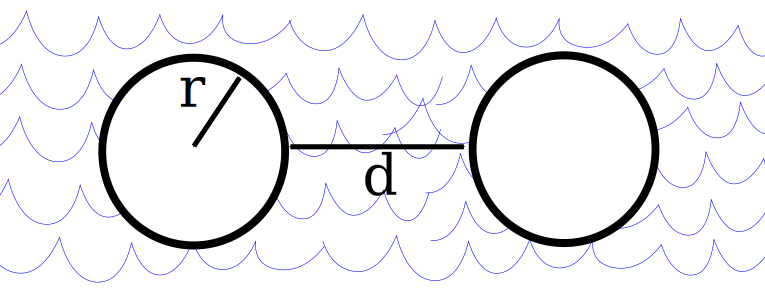
\includegraphics[width=3.5in]{figs/rods-diagram}
%\end{center}
%\caption{ Cross section schematic for two hydrophobic rods immersed in water.
%The radius and separation are shown.}
%\label{fig:rods}
%\end{figure}

\begin{figure}
\begin{center}
\includegraphics[width=3.5in]{figs/density-rods-in-water}
\end{center}
\caption{ Density profiles illustrating the transition from vapor 
to liquid water between the rods. The radius is 0.6~nm, the top figure is
at a separation of 0.6~nm and the
bottom is 0.7~nm. Figure~\ref{fig:rods-energy-vs-distance} shows
the energy for these and other separations.}
\label{fig:density-rods}
\end{figure}

To understand this critical separation, we consider the free energy in
the macroscopic limit, which is given by
\begin{equation}
F = \gamma A + pV.
\end{equation}
The first term describes the surface energy and the second term is the
work needed to create a cavity of volume $V$. Since the pressure term
scales with volume, it can be neglected relative to the surface term
provided the length scale is small compared with $\gamma / p$, which
is around $20~\mu m$, and is much larger than any of the systems we
study. For micron-scale rods, the water on the sides of the `stadium'
configuration will bow inward between the rods and the density will
reduce to vapor near the center point where the rods are closest to
each other.

Starting from the surface energy term, we can calculate the 
free energy per length, which is equal to the circumference multiplied 
by the surface tension. 
Working out the circumference of the stadium-shape leads us to
\begin{equation}
F = (2\pi r +4r+2d)\gamma
\end{equation}
where $\gamma$ is the surface tension, $r$ is the radius of the rods,
and $d$ is the separation between rods illustrated in
Figure~\ref{fig:density-rods}.  The force per length is the derivative
of the free energy with respect to the separation $d$, from which we
conclude that the force per length is twice the
surface tension.

We plot in Figure~\ref{fig:rods-energy-vs-distance} the computed free
energy of interaction
per unit length from our classical density functional (solid lines),
as a function of the separation $d$, along with the free energy
predicted by our simple macroscopic model (dashed lines).  The models
agree very well on the force between the two rods at close
separations, and have reasonable agreement as to the critical
separation for rods greater than 0.5~nm in radius.

\begin{figure}
\begin{center}
\includegraphics[width=3.5in]{figs/rods-energy-vs-distance}
\end{center}
\caption{ Free energy of interaction (also known as the potential of mean force)
versus separation for two hydrophobic rods ranging in radius from
0.2~nm to 1.2~nm.
All were arbitrarily offset to zero at large separations for ease of comparison. The
transition corresponds to the phase change from
vapor to liquid between the rods as pictured in the density profiles in 
Figure~\ref{fig:density-rods}. }
\label{fig:rods-energy-vs-distance}
\end{figure}

Walther \emph{et al}\cite{walther2004hydrophobic} studied the
interactions between two carbon nanotubes, which are geometrically
similar to our hydrophobic rods, using molecular dynamics with the SPC
model for water.  Their simulations used nanotubes of diameter 1.25~nm
and separations ranging from about 0.3~nm to 1.5~nm.  In agreement
with our findings for two purely hydrophobic rods, Walther \emph{et
  al} find that in the absence of Lennard-Jones attraction between
carbon and oxygen, there is a drying transition at a distance
comparable to the diameter of the nanotube.  In contrast to this, when
the attraction between nanotubes and water is turned on, they find
that the drying transition occurs at much shorter distances,
comparable to the diameter of water.

\subsection{Hydrophobic interactions of four rods}

\begin{figure}
\begin{center}
\includegraphics[width=3.5in]{figs/four-rods-energy-vs-distance}
\end{center}
\caption{ Free energy of interaction
versus separation for four hydrophobic rods ranging in radius from
0.2~nm to 1.2~nm.
All were arbitrarily offset to zero at large separations. The
transition corresponds to the phase change from
vapor to liquid between the rods as pictured in the density profiles in 
Figure~\ref{fig:density-four-rods}. }
\label{fig:four-rods-energy-vs-distance}
\end{figure}

\begin{figure}
\begin{center}
\includegraphics[width=3.5in]{figs/density-four-rods}
\end{center}
\caption{ Density profiles illustrating the transition from vapor 
to liquid water between four rods. The radius is 0.6~nm, the top figure is
at a separation of 1.53~nm and the
bottom is 1.56~nm. Figure~\ref{fig:four-rods-energy-vs-distance} shows
the energy for these and other separations.}
\label{fig:density-four-rods}
\end{figure}

We go on to study four parallel hard rods, as examined by Lum,
Chandler and Weeks in their classic paper on hydrophobicity at small
and large length scales~\cite{lum1999hydrophobicity}.  As in the case
of two rods---and as predicted by Lum~\emph{et al}---we observe a
drying transition, as seen the density plot shown in
Figure~\ref{fig:density-four-rods}.  In
Figure~\ref{fig:four-rods-energy-vs-distance}, we plot the free energy
of interaction together with the macroscopic approximation, and find
good agreement for rods larger than 0.5~nm in radius.  This free
energy plot is qualitatively similar to that predicted by the LCW
theory~\cite{lum1999hydrophobicity}, with the difference that we find
no significant barrier to the association of four rods.

\subsection{Hydration energy of hard-sphere solutes}

\begin{figure}
\begin{center}
\includegraphics[width=3.5in]{figs/sphere-energy-vs-diameter}
\end{center}
\caption{ Excess chemical potential per area versus radius for
  a single hydrophobic sphere
  immersed in water. This should have an asymptote equal to the
  surface tension at room temperature, and it agrees well with the
  surface tension in Figure~\ref{fig:surface-tension}. Results from a
  simulation of SPC/E water~\cite{huang2001shs} are shown as circles.
  The horizontal lines show the experimental and SPC/E macroscopic surface
  tension for water at standard atmospheric temperature and
  pressure. }
\label{fig:sphere-energy-vs-diameter}
\end{figure}

A common model of hydrophobic solutes is the hard-sphere solute, which
is the simplest possible solute, and serves as a test case for
understanding of hydrophobic solutes in
water\cite{sedlmeier2011entropy}.  As in the single rod, we begin by
examining the ratio of the excess chemical potential of the cavity
system to the solvent accessible surface area
(Figure~\ref{fig:sphere-energy-vs-diameter}).  This
effective surface tension surpasses the macroscopic surface tension at a
radius of almost 1~nm, and at large radius will drop to the macroscopic value.  As
with the single rod, we see the analytically correct behavior in the
limit of small solutes.  For comparison, we plot the free energy
calculated using a molecular dynamics simulation of SPC/E
water\cite{huang2001shs}.  The agreement is quite good, apart from the
issue that the SPC/E model for water significantly underestimates the
macroscopic surface tension of water at room
temperature\cite{vega2007surface}.

Figure~\ref{fig:density-sphere} shows the density profile for several
hard sphere radii, plotted together with the results of the same
SPC/E molecular dynamics simulation shown in
Figure~\ref{fig:sphere-energy-vs-diameter}\cite{huang2001shs}.  The
agreement with simulation is quite reasonable.  The largest
disagreement involves the density at contact, which according to the
contact value theorem cannot agree, since the free energies do not
agree.

\begin{figure}
\begin{center}
\includegraphics[width=3.5in]{figs/density-sphere}
\end{center}
\caption{ Density profiles around hard-sphere solutes of different radii. Predictions
  from our classical density-functional theory are in solid red, while
  the dotted line shows the result of a molecular dynamics simulation
  of SPC/E water~\cite{huang2001shs}.  }
\label{fig:density-sphere}
\end{figure}

\section{Conclusion}

We have developed a classical density functional for water that
combines SAFT with the fundamental-measure theory for hard spheres,
using one additional empirical parameter beyond those in the SAFT
equation of state, which is used to match the experimental surface
tension.  This functional does \emph{not} make a local density
approximation, and therefore correctly models water at both small and
large length scales.  In addition, like all FMT functionals, this
functional is expressed entirely in terms of convolutions of the
density, which makes it efficient to compute and minimize.

We apply this functional to the case of hard hydrophobic rods and
spheres in water.  For systems of two or four hydrophobic rods
surrounded by water, we see a transition from a vapor-filled state a
liquid-filled state.  A simple model treatment for the critical
separation for this transition works well for rods with diameters
larger than 1~nm.  In the case of spherical solutes, we find good
agreement with SPC/E simulations.

\bibliography{paper}% Produces the bibliography via BibTeX.

\end{document}
